\chapter{Background and Related work}
\label{chp:background}

In this chapter we provide a brief discussion of the essential background needed throughout the thesis. We will start by explaining the process of oil formation. Then we will explain the theory behind \gls{cnn} and their different optimization. To conclude, we will describe some data augmentation techniques and presented previous work that has been done in the use of deep learning in the field of geology.


\section{Geology}
The search for hydrocarbons - oil and gas - concentrates within the upper crust of the Earth which spreads from 0 to 40km. It is made of 12 tectonic plates that drifts away from each other. As they move, the plates interact at their extremities: creating and destroying material. During this process, minerals go through different phases (liquid, solid, gas). They are combined with a range of other minerals creating different rock types: it is the rock cycle. 
	\begin{figure}[!htp]
    \centering
        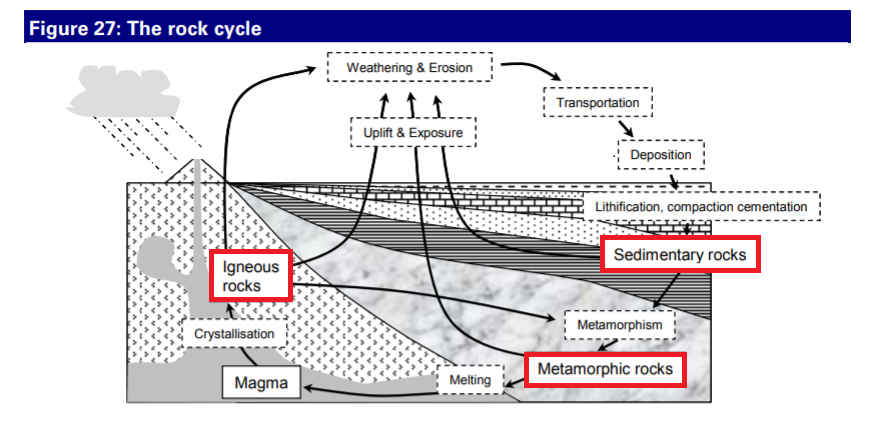
\includegraphics[width=1\textwidth]{figures/02-rock-cycle}
        \caption[The rock cycle]{The rock cycle describes how rocks transforms. It shows how erosion and weather transform igneous rocks in to sedimentary rocks. It further shows how metamorphism transforms the latter in metamorphic rocks. And how the crystallization of the magma of those produces igneous rocks. Adapted from the Oil and Gas beginners book \cite{oilbegin} }\label{fig:rock-cycle}
    \end{figure}

These cycles, and their interaction with biological processes form hydrocarbon source rocks, reservoir and seals. The movement of the plates also introduces non-linearity such as faults in the rocks where oil or gas can be trapped. Those structural traps are where we usually drill from. As we see in red in Figure~\ref{fig:rock-cycle}, there are three types of rocks: igneous, sedimentary and metamorphic. The cooling of minerals from magma  forms  igneous rocks. Metamorphic rocks are generated through  the burial process of rocks. As rocks are buried, they are exposed to higher temperature and pressure transforming organic matter into oil and gas. Sedimentary rocks account for almost all oil and gas reserve. They deposit in layers, reflecting the history of the depositional basin.


The hydrocarbon formation process has several steps. First the maturation. Organic matter is buried and exposed to such temperature and pressure conditions that it converts into hydrocarbon. Then follows the second part of the process: migration. It is when the hydrocarbon moves from the source rocks to the reservoir. The generated hydrocarbons have a lower density than the surrounding water, and at sufficient temperatures their viscosity is lowered (possibly even entering a gaseous phase) allowing them to move upwards through fractures in the source rocks and enter the permeable reservoir rocks. When it moves upwards, the pressure decreases causing it to condensate back to liquid form. The hydrocarbon is then trapped in the reservoir rock. The trap should ideally be impermeable (no fluid can flow through it). But an escape rate smaller than the production rate is sufficient for the trap to be commercially viable \cite{oilbegin}. 

Only a portion of this volume of hydrocarbon can be extracted. The amount depends on several factors such as porosity, permeability, lithology, etc...  The following sections present some of those properties. 
\subsection{Dunham Classification}
The Duhnam classification was developed to classify carbonate sedimentary rocks. The class names describe the depositional texture. This means that this classification is most significant for the interpretation of the depositional environment of the rocks. The Dunham classification, see Figure~\ref{fig:dunham}, follows three criteria: the supporting fabric of the original sediment (mud, grain, etc.), the presence or absence of mud, whether the original components were bound during deposition \cite{dunhamrevised}.
Those criteria lead to four classes :
\begin{itemize}
    \item \gls{ms}: mud-supported carbonate rock with less than 10\% grain.
    \item \gls{ws}: mud-supported carbonate rock with more than 10\% grain.
    \item \gls{ps}: grain-supported carbonate rock with more than 10\% mud.
    \item \gls{gs}: grain-supported carbonate rock with less than 10\% mud.
	\begin{figure}[!htp]
    \centering
        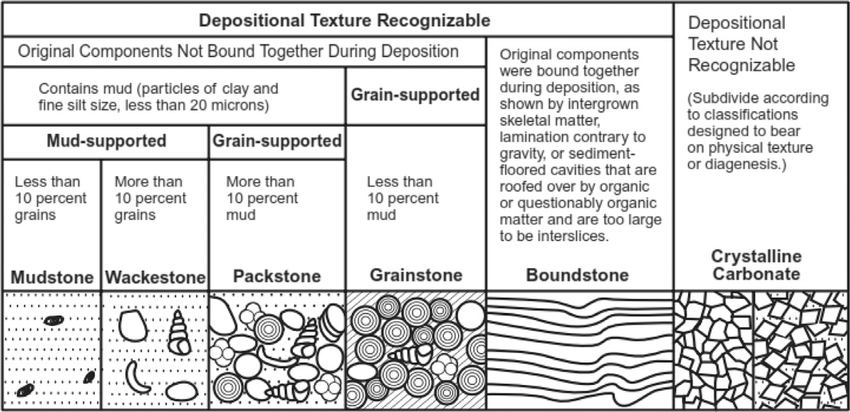
\includegraphics[width=1\textwidth]{figures/02-Dunhams-classification}
        \caption[Dunham Classifcation]{Dunham Classifiaction of carbonate rocks taken from Carbonate Calcium \cite{dunhamfig}}\label{fig:dunham}
    \end{figure}
\end{itemize}
In order to able to describe all carbonates rocks, Dunham defined two additional lithologies: 
\begin{itemize}
    \item Boundstone: if there is any evidence that sediments were bound at the time of deposition
    \item Crystalline Carbonate: re-crystallization has made it impossible to to identify the original carbonate texture.
\end{itemize}

This is a relevant property for reservoir rocks because it indicates what kind of rock it is: if it is going to be soft or hard to drill through etc.

\subsection{Porosity and Permeability}

The porosity of a rock is a measure of its ability to hold fluids. This is a relevant property for reservoir rocks since it will tell how much oil they can contain. We calculate the porosity by dividing the volume of open spaces in the rock by the total volume of the rock. Porosity is expressed by a number between 0 and 1. If the porosity is 0, then the rock can not hold any fluid \cite{oilbegin}. 
 
There are two kinds of porosity:
\begin{itemize}
    \item Total porosity: it includes all void spaces regardless of whether the pores are connected or isolated.
    \item Effective porosity: it is the fraction of the total volume in which fluid effectively flows. It includes dead-ends pores but excludes non-connected pores. This is the porosity that is most relevant in petroleum studies. 
\end{itemize}

The permeability of a rock describes how easily liquids can flow through it. It is an important property for the source rocks since hydrocarbon flows through them during the migration process. But it is also important for reservoir rock since if there is low permeability, the oil contained in the pores will not be able to flow out of the rock. 
Rocks that  combine good porosity and permeability are good reservoirs . Typically, rock with high porosity and high permeability will make a good reservoir rock. It can hold and deliver large amounts of oil. 

\subsection{Coring}\label{sec:coring}
The first step to determine where to drill is the seismic study. A big "bang" sends wave sounds that propagate into the earth crust and are partially reflected by the different rock layers. Geophones placed on the surface gather, register and store those wave sounds. This operation is repeated several times in different places and the data gathered creates a seismic images. This images are then interpreted by geologists to identify and target zones with high chances of finding oil \cite{oilbegin}. 


Once we found an area of interest, we drill a hole and lower sensors through the well to take measurements. Several instruments are used to collect those measurements.  Gamma ray gives information about the level of clay, resistivity indicates potential hydrocarbon sources and sonic indicates porosity of the rock. But the best way to identify what kind of rocks we drill through is coring. This operation consists in drilling very slowly with a special drilling bit and extract a piece of the rock which looks like a cylinder. Then we infiltrate a resine through the core to make sure it holds and all the fragments stick together. Then we cut very thin sections out of the core, take high resolution pictures, and we ask geologist to label them. The result is a precise description of the rock the exploration is drilling through \cite{oilbegin}.  

This technique is costly since it takes days out of the normal drilling process and it can be very slow. There can also be gaps in the core, it can collapse or sometimes we do not manage to extract core at all. This is why coring is not performed often. 

\section{Convolutional Neural Networks}
In the last couple of years, most of the best performing networks in image classification have been \gls{cnn} \cite{resnetpaper, alexpaper, googlepaper}. Some of them even surpassed human accuracy for normal images \cite{humanDNN}.
A \gls{cnn} is a network that makes the explicit assumption that its inputs are ordered. A rule of thumb, if shuffling the columns of the input does not influence the results of the network, we should not use \gls{cnn}s on this data. So the typical data used for \gls{cnn}s are images and text. 
For images, the ordered aspect of the data implies that one can encode some properties into the architecture of the network. One of them is that nearby pixels are more correlated than distant pixels. This allows the network to extract local features dependant only on small sub-regions of the image and it drastically reduces the number of parameters. 


A \gls{cnn} consists of three basic types of layers \cite{deepbook}.  In the first layer, several linear operations are performed in parallel. It produces a set of linear activation: it is the convolution layer. The second layer is the activation layer: the activation function is applied to the linear activation. This will produce a feature map representing the local features that were detected in the previous stage. The third layer is the pooling layer, this reduces the number of parameters to increase efficiency and produces a smaller feature map. Lastly, we can add a last layer: the fully connected layer, it will use the extracted features to classify the images into classes.


\subsection{Convolution Layer}

The convolution is performed on the input data by a filter or a kernel to produce a feature map. We proceed to the convolution by sliding the filter over the input. The convolution result is the summation of an elementwise multiplication between the input and the kernel. This results is written on the feature map. Each filter is trained to identify a certain feature and it will detect it everywhere on the image.  Many convolutions are performed using different kernels and producing several feature maps \cite{nnbook}.

Here is an example of how the feature maps are calculated. In Figure~\ref{fig:convo_calc}, the blue 3x3 matrix is the filter and the matrix on the left is the input. To get the 4 that is highlighted with green, we do an elementwise multiplication followed by a sum: 1x1 + 0x0 + 0x1 + 1x0 + 1x1 + 0x0 +1x1 + 1x0 + 1x1 = 4. 
	\begin{figure}[!htp]
    \centering
        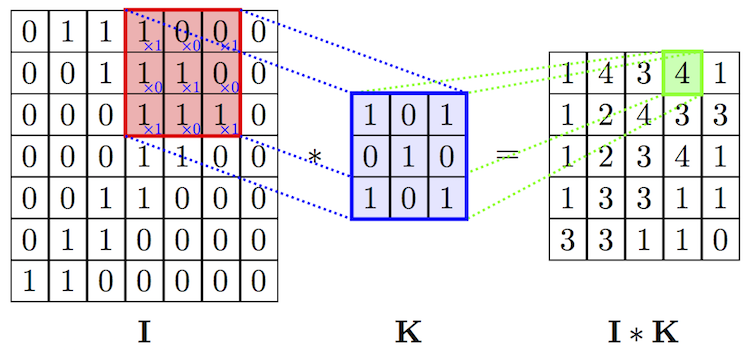
\includegraphics[width=0.9\textwidth]{figures/02-conv_layer}
        \caption[Convolution calculations]{Convolution layer calculations. The calculations are detailed above. Here the filter size is 3x3 and the stride is 1 since we are writing the 4th entry in the feature map.}\label{fig:convo_calc}
    \end{figure}
    
The area marked  in  red in the input is the receptive field. The kernel is moving over the image with a certain step size called the stride. A stride of 1 means that the kernel slides pixel by pixel. The stride length affect the size of the feature map: the larger stride length the fewer hidden neurons in the feature map. But no matter the stride size, the feature map will always be smaller than its input. This implies that if the network is deep, the feature maps might shrink. To prevent that, we use padding, which is adding a layer of zero value pixels to surround the input with. This keeps the spatial size constant after the convolution. It also improves the performance by preventing the information at the borders from being "washed away" and makes sure the kernel and stride size fit with the input \cite{cs231n}. 

\subsection{Pooling Layer}
After a convolution layer, it is normal to add a pooling layer. The purpose of pooling is to reduce the number of parameters and computations in the network. This shortens training and controls \gls{over-fitting}.
The type of pooling that is mostly used is max pooling which takes the largest value in each square as shown in Figure ~\ref{fig:maxpool}. The square dimensions (2x2 in Figure ~\ref{fig:maxpool})  and the stride are determined beforehand. This layer decreases the feature map size while keeping a sufficient amount of information. 
	\begin{figure}[!htp]
    \centering
        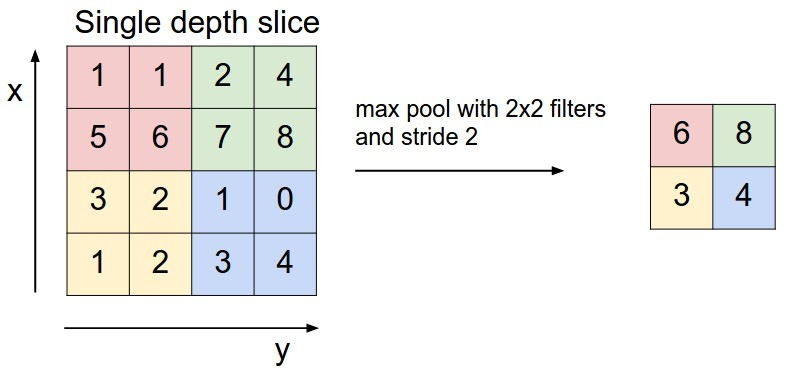
\includegraphics[width=0.9\textwidth]{figures/02-maxpool}
        \caption[Max Pooling layer]{Max pooling layer. We have a 2x2 filter with stride 2. We apply it to the output of the previous layer and it takes the maximum value of each 2x2 window. Taken from the Stanford course on \gls{cnn}s \cite{cs231n}}\label{fig:maxpool}
    \end{figure}
 
   
Most of the pooled output values have very small translational variance. This means that a translation in the input will not impact the output too much. This is very valuable since it is more important to detect the feature than to know precisely where it is situated in the image. The max-pooling will forget the exact position to focus on the relative position compared to the other features \cite{cs231n}.

\subsection{Classification Layer}
\label{sec:class_lay}
After the pooling layer, most \gls{cnn} architecture will have one or more fully connected layers. Those layers are connected to all the input neurons. To perform the classification, we need this fully connected layer to have as many output neurons as classes to classify. If you are trying to classify between red and white for example, you would have two output neurons.  It also needs to be combined with an activation function. This way, it outputs a probability distribution that allows the network to predict the class that has the highest probability. The choice of the activation function depends on the nature of the classification task \cite{deepbook}.
\subsubsection{Single label classification}
When a network is trying to predict only one class, we usually use a softmax activation function. It is defined as follows:
\begin{equation}
    softmax_j(x) = \frac{e^x_{j}}{\sum\nolimits_{k} e^x_{k}}
\end{equation}
Where \(x_j\) is the probability of the vector x to belong to class j. Softmax is useful because it converts the output of the last layer in the network into normalized class probabilities. The probabilities sums up to one. It makes it easy to identify the most likely output since it will be the one with the highest probability. 
\subsubsection{Multi-label classification}
The specific property of softmax that makes the probability sum up to 1 makes it unusable for multi-label classifications. Which is when one picture can have several labels. For that case, we use the sigmoid function as activation for the last layer. It will produce values between 0 and 1.
\begin{equation}
    sigmoid(x) = \frac{1}{1 - e^x} 
\end{equation}

The high values of output will be interpreted as high probability. We can choose a threshold for label selection, for example 0.5. We then say that if the value for the output of the sigmoid is greater than 0.5, we predict the label, otherwise we do not. This allows several labels to be predicted since more than one label can have a high value. 

\section{Optimization}
The aim of the training and optimization process is to tune the network's parameters in order to efficiently predict labels. To do that, we need to define an objective function which value measures the error between the prediction and the label. During the optimization, we use several methods to adjust the parameters to minimize the objective function.

\subsection{Losses} \label{sec:loss}
%%Editing note: (REF : \url{https://ml-cheatsheet.readthedocs.io/en/latest/loss_functions.htm}l)
We use two different objective functions in this thesis. The cross-entropy for single label classification and the binary cross entropy for multi-label classification. We will also refer to it as the loss. 
For single label classification, we define the cross-entropy loss as follows:
\begin{equation}
    H_y'(y) = - \sum\nolimits_k y'_k log(y_k)
\end{equation}

Where \(y_k\) is the predicted probability for class k and \(y'_k\) is the true probability for this class. It measures the performance of a classification which outputs probabilities between 0 and 1. On  Figure~\ref{fig:CE} , we can see that the closer we get to the true label, the smaller the loss. But when the probability decreases, the loss increases very quickly. So prediction that are very confident but wrong are more penalized \cite{nnbook}.
\begin{figure}[!htp]
    \centering
        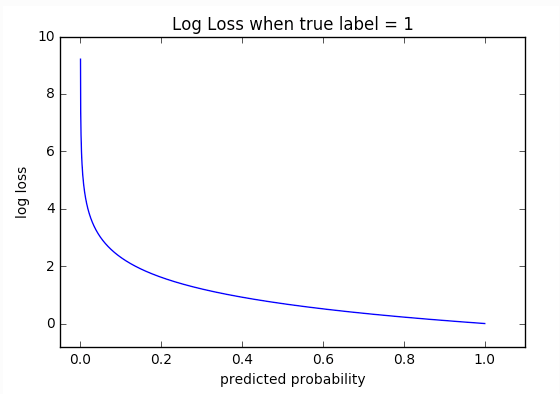
\includegraphics[width=0.9\textwidth]{figures/02-cross_entropy}
        \caption[Cross Entropy loss behaviour]{Cross Entropy loss behaviour. When we get close to the good prediction, the loss decreases slowly. But when we get further, the loss increases quickly. Plot taken from \cite{celoss}}
        \label{fig:CE}
\end{figure}


For multi-label classification, we use the binary cross entropy loss. That is because we are not treating our labels as integers, but as their one hot encoded representation. For single-labels, if we have three classes, label for class 1 will be 1, label for class 2 will be 2 etc.  For multi-label, we need to have the ability of having more than one label. A label for class 1 will then be [1, 0, 0], label for class 2 [0, 1, 0] and if an item is in class 1 and 2 its label will be [ 1, 1, 0]. In the case the values of \(y'_k\) are 0 or 1, we use binary cross entropy loss which is defined as follows: 
\begin{equation}
    H_y'(y) = - \sum\nolimits_k y'_k log(y_k)\ + (1 - y'_k)log(1 - y_k)
\end{equation}


Those are basically two different formulation of the same loss. They have the same behavior and can both be referred to as log loss. 
\subsection{Gradient Descent and Learning Rate} \label{sec:grad_lr}
%% Editing note: . LEX FRIDMAN MIT
%% Editing note: RF : https://towardsdatascience.com/gradient-descent-in-a-nutshell-eaf8c18212f0
 \begin{quote}
     "A gradient measures how much the output of a function changes if you change the input a little bit."
 \end{quote} Lex Fridman, MIT. 


In order to minimize the objective function, we use gradient based methods. The gradient descent is an iterative method which updates the parameters of the network with the aim of minimizing the objective function. By moving the parameters in small steps in the opposite direction of the gradient, we reduce the objective function \cite{cs231n}. 

Let J(\(\theta\)) be our objective function and \(\theta\) the parameters of the network. The gradient descent updates the parameters as follow: 
\begin{equation}
    \theta' = \theta - \eta . \nabla_\theta J(\theta)
\end{equation} The learning rate \(\eta\) determines the impact of these updates on the parameters. \(\nabla_\theta J(\theta) \) is the gradient of the objective function. At every iteration, the objective function is one step closer to the local minimum. The size of this step is influenced by the learning rate, but also by the objective function itself: a big loss will result in big updates. 


The learning rate plays a crucial role: if it is too high, the learning might miss the local minimum and if it is too small, learning might be very slow. In both cases the biggest risk is that our function never converges to its local minimum. Either because it keeps bumping on the gradients convex function or because it takes too long, see Figure~\ref{fig:LR}  \cite{cs231n}.  
\begin{figure}[!htp]
    \centering
        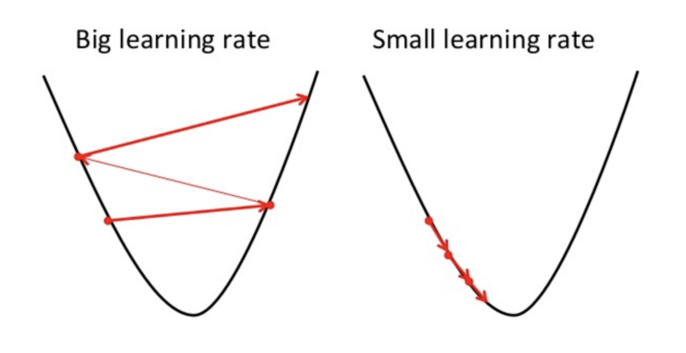
\includegraphics[width=1\textwidth]{figures/02-LR}
        \caption[Gradient behaviour for different learning rates]{Gradient behaviour for different learning rates. On the left, the learning rate is too big so the gradient bounces back and forth on the function. On the right it is too small so it converges very slowly towards the minimum. Figures taken from \cite{gradient} }
        \label{fig:LR}
\end{figure}

Figure~\ref{fig:LR_impact} shows the different behaviours of the training loss based on the value of the learning rate. The yellow curve shows a very high learning rate. The loss increases quickly, the gradient has taken such a big step that it most likely exited the local minimum and it can not converge. The green curve shows a bit smaller learning rate. The gradient goes down the curve but then bounces back and forth on the gradient curve as in Figure~\ref{fig:LR}. It will converge to a non optimal value of the loss. Then the blue curve shows a small learning rate. The gradient updates the weight too slowly and they are not corrected enough to reach the optimal loss value in time. Lastly, the red curve shows a good learning rate. Early in the training, we take big steps in the gradient so the loss decreases quickly. But when we are close to the local minimum, the steps are smaller and the loss converges \cite{lr}. 

%% Editing note :  RF :https://towardsdatascience.com/understanding-learning-rates-and-how-it-improves-performance-in-deep-learning-d0d4059c1c10
There are different strategies to choose the good learning rate. A general idea is to start with a big learning rate to learn quickly in the beginning and make it smaller as we go along with the training. 
\begin{figure}[!htp]
    \centering
        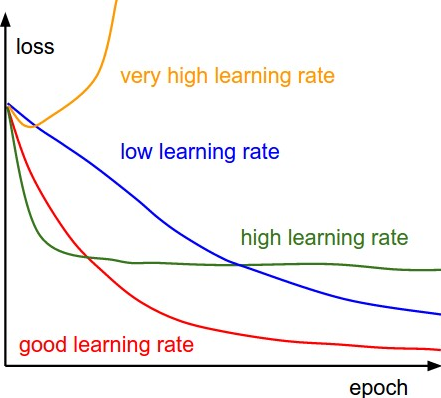
\includegraphics[width=0.7\textwidth]{figures/02-LR_impatc_train}
        \caption[Impact of the learning rate on training]{Training loss evolution based on different values of the learning rate. This image has been taken from \cite{cs231n}}\label{fig:LR_impact}
\end{figure}

\subsection{Gradient Descent Variants}
There are three variants of gradient descent which differ in the amount of data we use to compute the gradient of the cost function \cite{gradient}. 
\begin{itemize}
    \item The batch gradient descent compute the gradient of the cost function for the entire training dataset. This is computationally efficient and gives a stable error gradient but it is intractable if the dataset does not fit in memory. 
    \item The second variant is \gls{sgd} which computes the gradient for every training example. It can be redundant since we recompute the gradient for very similar training examples.
    \item The third variant is a compromise between the two others, it computes the gradient for every mini batch of n training example. This reduces the variance of the parameter update without wasting computation. It can also lead to a more stable convergence.
\end{itemize}There are still challenges, mainly regarding the learning rate. As we stated earlier, it is difficult to find a good value for it. A solution is to reduce the learning rate according to a specific time line. We may reduce it by a factor of 10 every tenth epoch, for example, or when the cost function is below a fixed threshold. These strategies are effective but they have to be defined in advance so they don not adapt to the data. The ultimate challenge is to keep the gradient from getting stuck in local minimun or saddle points. Some algorithms or additional parameters have been implemented to overcome those challenges
\subsection{Momentum}
Around a local minimum, the surface curves are often steeper in one dimension than the others, this is called a ravine. In those areas, the gradient descent oscillates across the slopes and converges slowly to the local minimum. The momentum helps to achieve convergence faster by speeding up the gradient descent in the good direction. For that, it remembers the value of the update vector at the past iteration and uses it to calculate the new update \cite{optimgrad}. 
\begin{equation}
    v_t = \gamma v_{t-1} + \eta . \nabla_\theta J(\theta)
    \theta' = \theta - v_t
\end{equation}
\begin{equation}
    \theta' = \theta - v_t
\end{equation}
Where \(v\) is the velocity and \(\gamma\) is the momentum term. The velocity represents the direction and the speed of the parameters. \(\gamma\) determines how much the velocity term impacts the update. With momentum, the gradient keeps in memory the direction the gradient was going before. So if the gradient keeps going in the same direction, it will gain velocity and make bigger updates. But if there is a sudden change of direction, the update will be moderated and there will be less oscillations. A common analogy for this is to imagine a ball going down a hill. While it rolls down, the momentum adds mass, making it go faster and overcoming smaller bumps \cite{optimgrad}. A risk of this technique is that if the gradient accumulates too much velocity in one direction, it might overlook the minimum. 

\subsection{Adam Optimizer}

An other optimization algorithm is Adam and stands for Adaptive Moment Estimation. It computes adaptive learning rates for each parameter. Adam stores estimates of the first and second moments - \(m_t\) and \(v_t\) - which are respectively the mean and the uncentered variance of the gradient. They are computed as follows:
\begin{subequations}
\begin{align}
v_t & = \beta_2 v_{t-1} + (1 - \beta_2)g_t^2 \\
m_t & = \beta_1 m_{t-1} + (1 - \beta_1)g_t
\end{align}
\end{subequations}
Where \(\beta_1\) and \(\beta_2\) are the learning rates and \(g_t\) is the gradient. The parameter updates according to how much the gradients are changing on average but also from one iteration to the other.  \(m_t\) and \(v_t\) are initialized as 0 vectors. Experiments shows that they are biased towards 0, especially during the early steps when the learning rates are small. We handle this bias by producing estimates of the first and second moment that are bias corrected \(\hat{m}_t\) and \(\hat{v}_t\), \cite{adam}.
\begin{subequations}
\begin{align}
\hat{v}_t &=  \frac{v_{t}}{1 - \beta_2^t} \\ 
\hat{m}_t &=  \frac{m_{t}}{1 - \beta_1^t}
\end{align}
\end{subequations}

We then use those estimates to calculate the parameters update as follow: 
\begin{equation}
    \theta_{t+1} = \theta_t - \frac{\eta}{\sqrt{\hat{v}_t} + \epsilon}\hat{m}_t
\end{equation}
Where \(\eta\) is the general learning rate for the parameter update and \(\epsilon\) is a small constant to ensure mathematical stability. 
The detailed  Adam algorithm is presented in Figure \ref{fig:adam_algo}.
\begin{figure}[!htp]
    \centering
        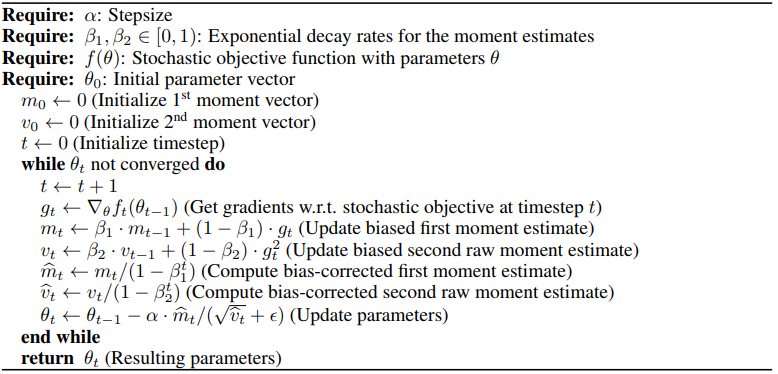
\includegraphics[width=1\textwidth]{figures/02-adam_algo}
        \caption[Adam Algorithm]{ This Algorithm is a optimization of the \gls{sgd}. It describes the update rule for the first and second moment. This algorithm has been taken from \cite{adam}}\label{fig:adam_algo}
\end{figure}
The Adam optimizer is an iterative algorithm. It means that the parameters will be updated until they reach the stopping criterion. 
Adam optimizer has shown that it achieves good results fast and is thus used as a default in many 
computer vision and deep learning algorithms. There are several variants of the Adam optimizer.

\subsection{Adamax}
One variant of the Adam algorithm is the Adamax optimizer. In the Adam algorithm, we use the \(L^2\) norm to update \(v_t\). This can be generalized to a \(L^p\) norm based update rule that would write as follows: 
\begin{equation}
    v_t = \beta_2^p v_{t-1} + (1 - \beta_2^p) \mid g_t\mid^p
\end{equation}
This variant will become unstable as p gets bigger than 1 or 2. Surprisingly, as \(p\to\infty\), the behavior is simple and stable. If we then define \(u_t\) as 

\begin{subequations}
\begin{align}
u_t & = \lim_{p\to\infty}(v_t)^{1/p} \\
u_t & = \lim_{p\to\infty}(\beta_2^p v_{t-1} + (1 - \beta_2^p)\mid g_t\mid^p)^{1/p} \\
u_t & = \lim_{p\to\infty}(1 - \beta_2^p)^{1/p}(\sum_{i=1}^{t}\beta_2^{t-i} \mid g_i\mid ^p)^{1/p} \\
u_t & = \lim_{p\to\infty}((1 - \beta_2^p) \sum_{i=1}^{t}\beta_2^{t-i} \mid g_i\mid ^p)^{1/p} \\
u_t & = \lim_{p\to\infty}(\sum_{i=1}^{t}\beta_2^{t-i} \mid g_i\mid ^p)^{1/p} \\
u_t & = \max (\beta_2^{t-1}  \mid g_1\mid, \beta_2^{t-2}  \mid g_2\mid ), ..., \beta_2^ \mid  g_{t-1}\mid, \mid g_t\mid
\end{align}
\end{subequations}
The last equation can be very easily written recursively: 
\begin{equation}
    u_t = \max(\beta_2 . u_{t-1},  \mid g_t\mid)
\end{equation}
As shown in Figure \ref{fig:adamax_algo}, \(u_t\) is initialized to 0 and then plugged in the Adam update: 
\begin{equation}
  \theta_{t+1} = \theta_t - \frac{\eta}{u_t} \hat{m}_t
\end{equation}

\begin{figure}[!htp]
    \centering
        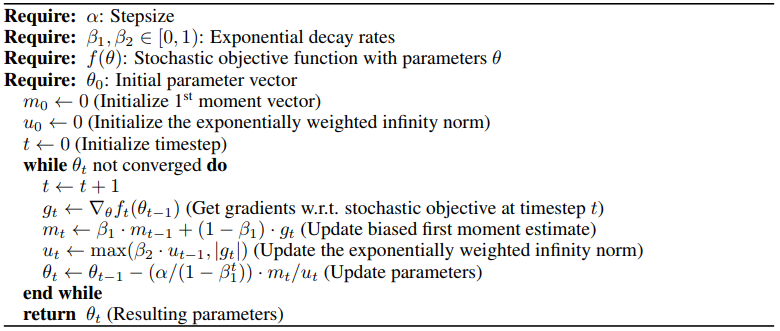
\includegraphics[width=1\textwidth]{figures/02-adamax_algo}
        \caption[Adamax Algorithm]{ This Algorithm is a variant from the Adam algorithm presented below. It is based on the infinity norm. The proof of why we use the max operation is explained in this section. This algorithm has been taken from \cite{adam}}\label{fig:adamax_algo}
\end{figure}

As \(u_t\) relies on the \(\max\) operation, it does not have a bias towards 0. This is why we do not need to calculate an estimate nor add a stabilization constant as for \(\hat{v}_t\) to calculate the update rule \cite{adam}.

\section{Accuracy and Validation metrics}
In order to find out how a model is performing, we need to choose some metrics. The most popular one is accuracy since it speaks to anyone even not familiar with the field. But it can be limited in some cases and give a false impression that the model is doing well when it actually is not. To get a better overview, we use precision and recall. 

\subsection{F1 score}
While accuracy is a good indication of how well the model is performing, they can give erroneous information. Let say you are trying to identify people with a rare disease. We could very easily produce a model with 99.999999\% accuracy to identify a healthy person simply by labeling every single individual as sick.We produced a model with a nearly perfect accuracy, but with no value. In cases where there is quit a big imbalance between classes, the accuracy will not be a good measure of performance.
What is important in our toy case is to identify as many of the relevant cases as possible, this is similar to maximizing the recall \cite{multimetrics}. 

Recall calculation uses true positive (samples classified as positive that are actually positive) and true negatives (samples classified as negative that are actually positive). The recall is then defined as the number of true positives divided by the sum of the true positives and false negatives \cite{metrics}. 
\begin{subequations}
\begin{align}
recall & = \frac{True Positives}{True Positives + False Negatives} \\
 & = \frac{Sick People Correctly Identified}{Actually Sick People}
\end{align}
\end{subequations}

But a model with very high recall will have a bad precision. We would not want to tell healthy people that they are sick. 

The precision focuses on the proportion of samples we said were correctly classified actually were. For that we introduce false positives (samples classified as positive that are actually negative). The precision is then defined as the number of true positives divided by the sum of true and false positives \cite{metrics}.
\begin{subequations}
\begin{align}
precision & = \frac{True Positives}{True Positives + False Positives} \\
 & = \frac{Sick People Correctly Identified}{People Identified As Sick}
\end{align}
\end{subequations}

 In cases where we want to find an optimal trade-off between precision and recall, we use the F1-score which is defined as: 
 \begin{equation}
     F1 = 2*\frac{precision * recall}{precision + recall}
 \end{equation}
 The precision is a measure of a classifier's exactness while recall is a measure of a its completeness. 
 We use a harmonic mean to avoid giving good F1 scores to models with extreme values: 1 of recall and 0 of precision for example \cite{wiki-f1}. 
In some cases, samples can have more than one labels, and the different classes can be unbalanced. A way to handle that is to calculate the F1 score by calculating it for each class.  Then we do a weighted sum to take into account classes that are more populated than others. 
There are several ways to visualize precision and recall, one of them is to use confusion matrices. 
\subsection{Confusion Matrix}
A confusion matrix is a an overview of the precision and recall results of a classification problem. The columns represent the number of occurrences of the predicted labels for each class. The rows represent the number of occurrences of the real labels for each class. It shows how the classification task is confused. This gives insight on the kind of error being made \cite{cm}. 

\begin{figure}[h]
    \centering
        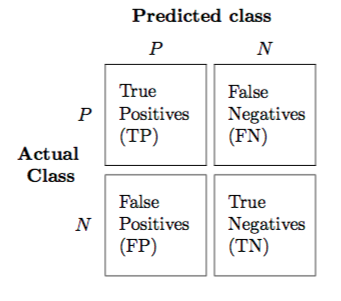
\includegraphics[width=0.5\textwidth]{figures/02-CM}
        \caption[Confusion matrix]{Confusion matrix for a binary classification. This is a good way to rapidly visualize true positives, false negatives... And it is also easy to calculate precision and recall. Figure taken from \cite{cm_image}}\label{fig:CM}
\end{figure}

It is relevant to know if your model is more likely to mix up  a German shepherd for a fox or a fox for a turtle. It makes the interpretation of the results better since you know how your model is biased. Also, some errors are more acceptable than others. We can consider a model with lower accuracy but miscalssifying similar objects better than a model with very high accuracy but missing simple cases. 
It makes it also easy to get the precision and the recall of the model. In Figure~\ref{fig:CM}, we see clearly how to identify true and false positives/negatives. This makes the calculation that we saw in last section easy to make. 

\section{State of the art networks}
We focus on three network architectures that have proven to give significant results in the classification task. Today, ResNet is the one that achieves the best results and AlexNet is the one that does it in the shortest time.    

\subsection{GoogLeNet and Inception\_v3}
GoogLeNet was the winner of the ILSRVC in 2014, it also known as Inception V1. It is a \gls{cnn} inspired by LeNet that introduces a new type of module called inception. Those modules can be seen as smaller models within the network. 

In classic architecture, you have to decide at each layer which size the filters for the convolution should be: 5x5, 3x3 etc. But from one image to another, the location of the information and its size can vary greatly. That is why it is difficult to know beforehand which of those convolutions would give the best result. The inception module tackles this problem by performing all the convolutions in parallel. It then concatenates the different feature maps before passing it on to the following layer. This way, the model can pick up both local features from the small convolutions and more general features with bigger convolutions \cite{googlepaper}. 

Figure~\ref{fig:inception} shows the detailed implementation of the inception module. As we explained before, 1x1, 3x3 and 5x5 convolutions are done in parallel. The max-pooling layer is added because it has been successfully used in most current state of the art networks. Also, a 1x1 convolution as well as a ReLu activation are added to reduce the dimensionality of the feature map. This way we reduce the number of parameters before passing it to the bigger convolutions. The GoogLeNet is 22 layers deep and stacks convolution layers and inception module as presented in Figure~\ref{fig:googl}.

\begin{figure}
\begin{subfigure}[b]{.8\textwidth}
  \centering
  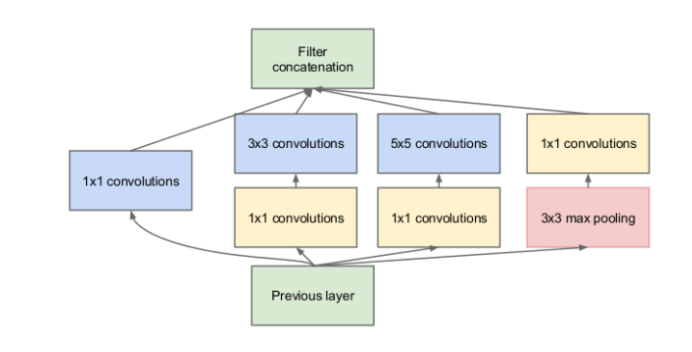
\includegraphics[width=1\linewidth]{figures/02-inception_module}
  \caption{The inception module with dimensionality reduction }
  \label{fig:inception}
\end{subfigure}
\\
\begin{subfigure}[b]{.8\textwidth}
  \centering
  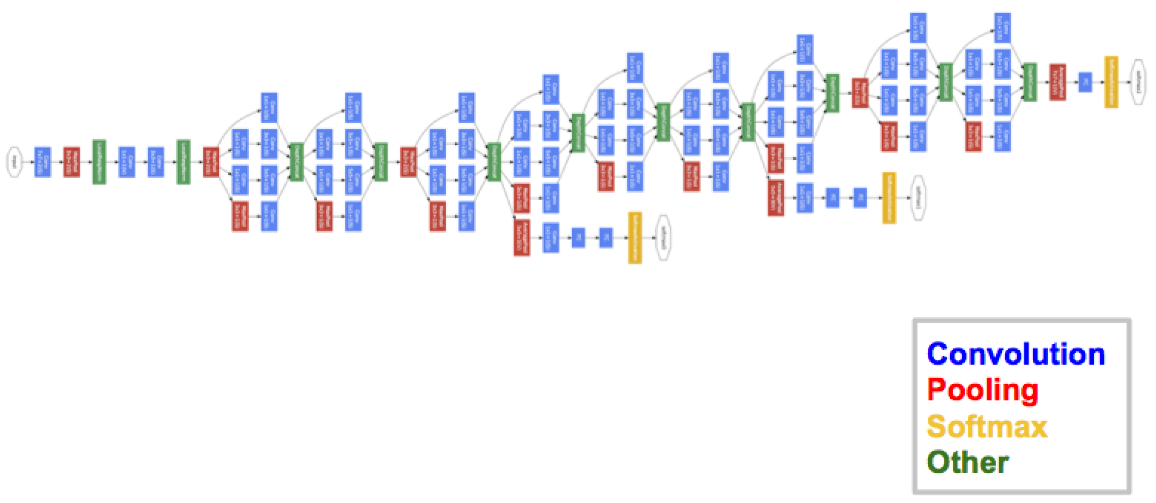
\includegraphics[width=1\linewidth]{figures/02-googlearch}
  \caption{Full 22-layers architecture of Inception\_v3}
  \label{fig:googl}
\end{subfigure}
\caption[Inception network architecture]{Detailed and overview of the architecture of Inception\_v3. Both images have been taken from the original paper \cite{googlepaper}}
\end{figure}
Some optimization were presented in \cite{googlepaper}. The first one is Inception-v2 which tackles the issue of representational bottleneck. This happens when one use reduces the dimension of the input too much resulting in a loss of information. It solves this issue by replacing the 5x5 convolution by two 3x3 convolutions, which also boosts the performance. On top of that Inception\_v3 implements a RSMSProp optimizer. It also performs a factorization of the 7x7 convolutions in a similar way as Inception-v2 and label smoothing. 

\subsection{ResNet}
ResNet won first place in the ILSRVC 2015 image classification competition. It introduces a new network architecture called residual learning. 

When deep networks get even deeper, the accuracy gets saturated and decreases rapidly: this is the degradation problem \cite{resnetpaper}. That is the issue residual learning aims to solve. This phenomenon is surprising since one would think that a network with extra layers would learn as much, if not more, than a shallower network. But experiments prove that this is not the case. Deeper networks gets a worse accuracy than shallower ones, see on the left of Figure~\ref{fig:resnetaccs}. The 34-layers plain network has a higher error than the 18-layers network. 

\begin{figure}[!htp]
    \centering
        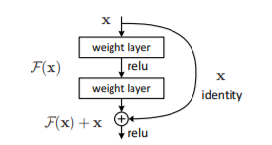
\includegraphics[width=0.9\textwidth]{figures/02-resnet_block}
        \caption[Building block of ResNet]{Building block of ResNet. Instead of having only stacked layers, we also have the identity function. Figure taken from the original paper \cite{resnetpaper}}\label{fig:resnetblock}
\end{figure}
%% Editing note : medium article 
A regular network architecture learns the mapping of input x to output y with a function H(x) which is a few stacked non linear layers. ResNet architecture defines a residual function using F(x) = H(x) – x which can be expressed as F(x) = H(x) + x. H(x) is a few stacked non linear layers and x is the identity function, see Figure~\ref{fig:resnetblock}. The intuition behind this architecture is that if the identity mapping is optimal (we want the input to be equal to the output), it is easier to drive H(x) to 0 and only keep the identity than to fit H(x) to the identity \cite{mediumresnet}. In practice, identity mappings are rarely optimal. But the hypothesis that it’s easier to optimize a residual mapping  than the original mapping is proven during experiments. Figure~\ref{fig:resnetaccs} shows that ResNet overcomes the degradation problem. It also achieves better results than its plains counterparts.


\begin{figure}[!htp]
    \centering
        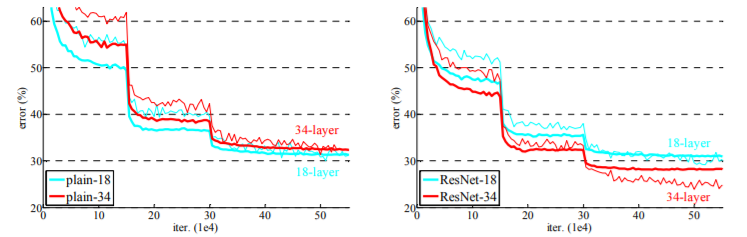
\includegraphics[width=1\textwidth]{figures/02-Resnet_comparing_acc}
        \caption[Degradation problem solved]{Training on ImageNet. Thin curves are training error, and bold curves are validation error of the center crops. Left: plain
networks of 18 and 34 layers. Right: ResNet of 18 and 34 layers. Taken from the riginal paper \cite{resnetpaper}}\label{fig:resnetaccs}
\end{figure}

\subsection{AlexNet}
AlexNet architecture focuses on parallelizing \gls{cnn}s across multiple GPUs. It won first place in the ILSRVC in 2012. It had a great impact on deep learning and computer vision since it allowed networks to scale better than all alternatives.
The idea is to parallelize in different ways depending on the kind of layer the network is training\cite{alexpaper}. There are two ways of parallelize the training of a network : 
\begin{itemize}
    \item Model parallelism: different workers train different parts of the model. The workers must synchronize whenever a model part trained by a worker needs output from another model part trained by an other worker.  
    \item Data parallelism: different workers train on different data samples. The workers must synchronize the model parameters to make sure they are learning a consistent model. 
\end{itemize}
As we saw in section 2.3, \gls{cnn}s consist of two types of layers. Convolutional layers that contain most of the computations (between 90 and 95\%) and fully connected layers that contains most of the model parameters (around 95\%). In AlexNet, the convolutional layers rely on data parallelism while fully connected layers rely on model parallelism \cite{alexpaper}. 

This is illustrated in Figure~\ref{fig:alexnet}. 
\begin{figure}[!htp]
    \centering
        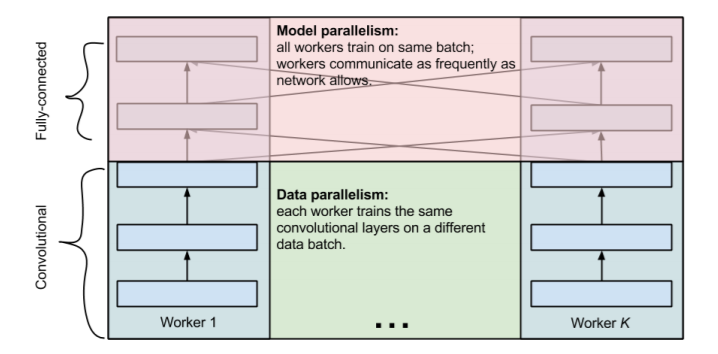
\includegraphics[width=0.9\textwidth]{figures/02-alexnet}
        \caption[AlexNet architecure overview]{Training of a network with 3 convolutional layers and 2 fully-connected layers by K workers. Taken from the original paper \cite{alexpaper}}\label{fig:alexnet}
\end{figure}
What happens is that each of the K workers is given different data batch and computes all the convolutions on its data: this is data parallelism. Then it switches to model parallelism. One worker sends its last staged convolution to all other workers.  Then it computes the fully-connected layers and start back propagation. In parallel, the next worker sends its last-stage convolution to all other workers. They can then compute the fully-connected layers on the second batch and so on. The same behavior is implemented in the back propagation. 

\subsection{Transfer Learning} \label{sec:translearn}
%% Editing note \url{https://arxiv.org/abs/1411.1792} 
%% Editing note: . \url{https://ieeexplore.ieee.org/stamp/stamp.jsp?arnumber=5288526}
%% Editing note: link to c231n course)
There are few database big enough to properly train those networks. And when there is, it can takes weeks before the network achieves acceptable results. A clever way to use those networks is through transfer learning. This technique relies on the fact that what a network learns from a data set is still useful for another data set \cite{translearnsurvey}. To transfer this knowledge,  we download the weights used to achieve the best performance of a network on an sufficiently big data set. Then we build our training algorithm on top of that network. A very important property underlying this is that the deeper the layers of a network, the more complex shapes the network learns \cite{layerslearn}. So the early layers learn the basic shapes, colors etc. while deeper layers learn complex shape, and more subtle variation in the image. 
There are two major ways of using transfer learning. 
\begin{itemize}
    \item Fine-tuning: The network is initialized - all the parameters of every layer - with the pretrained network. The network is in most case pretrained on the ImageNet data set on 1000 classes. It is just another way to initialize weights, nothing is changed further in the training algorithm \cite{cs231n}.
    \item Network acts as feature extractor: An other way to use it is to set all the weights to the pretrained ones. Then we freeze all the layers, except the final fully connected one. This last layer is initialized to random weights and only those weights are modified during the training. 
    This technique is quicker since gradients are only computed for the last layer
\end{itemize}
Those two techniques can be adapted.  An alternative would then be to freeze the k first layers and just learn again the n-k remaining ones to adapt it best to our classification task. For example, if the classification problem contains images that are  different to the ones contained in the ImageNet, we might want to retrain most of the model \cite{translearnsurvey}. 
Using transfer learning helps achieving faster and better results. Since it starts from a very advanced level instead of starting from scratch, the networks converges and learns much more quickly on the new data.

\section{Data Augmentation} \label{sec:dataug}
As mentioned in the section above, it is rare to find data sets big enough to train the state of the art networks. Fortunately a collection of methods known as data augmentation can artificially boost the size of small data sets. The aim is to create more training data from the ones that we already collected. The most common operations are rotations, flips, resizing, rescaling etc... Other techniques that changes the image a bit more can also be used.
\begin{itemize}
    \item Color Jitter: It is a gentle way to change the brightness, contrast, hue and saturation of the image. 
    For each parameter p, Color Jitter chooses a random value v between 1 - p and 1 + p and then applies the parameter adjustment with this value v. So for example, if we choose to set the brightness parameter to 0.3. The method will chooses a random value between 0.7 and 1.3, let say 1.05 and adjust the brightness with a intensity of 1.05. This is why it is important to keep the values small. Indeed, if we choose 0.8 for brightness for example, we risk to have it adjusted with an intensity of 0.2 which would result in an almost completely black image.
     \item Elastic Transform:   Elastic transformation relies on the fact  that images have some invariance to elastic deformation. Elastic deformation describes the temporary deformation of a material that will later regain its original form. Instead of moving the whole image as in affine transformation, we move each pixel to a new position dependent of the previous one \cite{elastic}. This can be seen as a grid underlying the image. Each point of the grid will be slightly moved, resulting in a distorted image. 
     \end{itemize}

\begin{figure}[!htp]
    \centering
        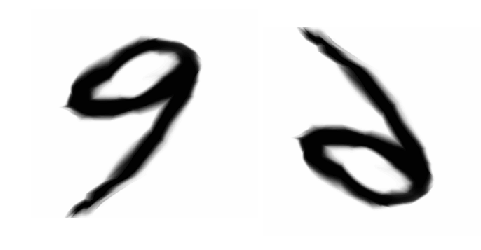
\includegraphics[width=1\textwidth]{figures/02-badaug}
        \caption[Data Augmentation Limitations]{Example of data augmentation changing the nature of the image. The flipping has changed the meaning of the image from 9 to 6. Taken from \cite{badaug_im}}\label{fig:badaug}
\end{figure}
     
Nevertheless, data augmentation should be used carefully. There is a risk that the image is transformed so much that it is not usable by the algorithm anymore. Figure \ref{fig:badaug} shows how flipping can change the meaning of the image and introduce error in the labels. 
\section{Related work}
Machine Learning and Deep Learning have been implemented in oil and gas companies for a range of uses. One of the applications is in the interpretation of seismic data. For instance, these papers \cite{dlseismiclitho, dlseismicfeatures} explains how we can use \gls{cnn} to predict lithology and geological features based in seismic data.  

An other use of Deep Learning in petroleum geoscience is in the interpretation of wireline log data. As we mentioned in section \ref{sec:coring}, once we identified regions of interest from seismic interpretation, we drill exploration wells. To get as much information as possible about what we drilled through, we lower several sensors into the well. The data gathered from those sensors is called wireline log data. For instance, we can apply Neural Networks to this data to determine the porosity the reservoir \cite{dlwirelineporo}, or determine the different rocks and their boundaries in the reservoir \cite{dlwirelinefacies}. 

We can also use Machine Learning to classify carbonates rocks from core samples \cite{carbo}. This paper showed that \gls{svm} and \gls{rf} classified carbonate sediments from core efficiently. We can also use Neural Networks to classify carbonate rocks according to the Dunham classification \cite{dltexture}. 
